\section{Relação: Algoritmos x Programas}

\begin{frame}{O que é um computador?}
  Um computador pode ser interpretado como uma máquina eletrônica programável capaz de processar dados, executar instruções e realizar tarefas específicas.  Ele é composto por hardware (parte física) e software (programas e instruções), trabalhando juntos para processar informações de maneira rápida e precisa \cite{medina2006algoritmos}.
  \begin{figure}
    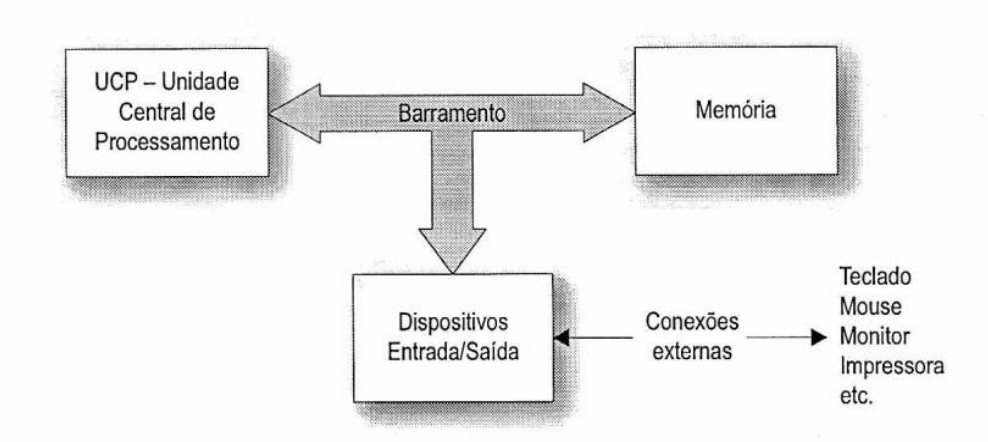
\includegraphics[width=0.5\textwidth]{figuras/Arquitetura.png}
    \caption{Arquitetura simplificada de um computador.}
  \end{figure}
\end{frame}